% !TeX program = pdfLaTeX
\documentclass[smallextended]{svjour3}       % onecolumn (second format)
%\documentclass[twocolumn]{svjour3}          % twocolumn
%
\smartqed  % flush right qed marks, e.g. at end of proof
%
\usepackage{amsmath}
\usepackage{graphicx}
\usepackage[utf8]{inputenc}

\usepackage[hyphens]{url} % not crucial - just used below for the URL
\usepackage{hyperref}

%
% \usepackage{mathptmx}      % use Times fonts if available on your TeX system
%
% insert here the call for the packages your document requires
%\usepackage{latexsym}
% etc.
%
% please place your own definitions here and don't use \def but
% \newcommand{}{}
%
% Insert the name of "your journal" with
% \journalname{myjournal}
%

%% load any required packages here


% Pandoc syntax highlighting
\usepackage{color}
\usepackage{fancyvrb}
\newcommand{\VerbBar}{|}
\newcommand{\VERB}{\Verb[commandchars=\\\{\}]}
\DefineVerbatimEnvironment{Highlighting}{Verbatim}{commandchars=\\\{\}}
% Add ',fontsize=\small' for more characters per line
\usepackage{framed}
\definecolor{shadecolor}{RGB}{248,248,248}
\newenvironment{Shaded}{\begin{snugshade}}{\end{snugshade}}
\newcommand{\AlertTok}[1]{\textcolor[rgb]{0.94,0.16,0.16}{#1}}
\newcommand{\AnnotationTok}[1]{\textcolor[rgb]{0.56,0.35,0.01}{\textbf{\textit{#1}}}}
\newcommand{\AttributeTok}[1]{\textcolor[rgb]{0.77,0.63,0.00}{#1}}
\newcommand{\BaseNTok}[1]{\textcolor[rgb]{0.00,0.00,0.81}{#1}}
\newcommand{\BuiltInTok}[1]{#1}
\newcommand{\CharTok}[1]{\textcolor[rgb]{0.31,0.60,0.02}{#1}}
\newcommand{\CommentTok}[1]{\textcolor[rgb]{0.56,0.35,0.01}{\textit{#1}}}
\newcommand{\CommentVarTok}[1]{\textcolor[rgb]{0.56,0.35,0.01}{\textbf{\textit{#1}}}}
\newcommand{\ConstantTok}[1]{\textcolor[rgb]{0.00,0.00,0.00}{#1}}
\newcommand{\ControlFlowTok}[1]{\textcolor[rgb]{0.13,0.29,0.53}{\textbf{#1}}}
\newcommand{\DataTypeTok}[1]{\textcolor[rgb]{0.13,0.29,0.53}{#1}}
\newcommand{\DecValTok}[1]{\textcolor[rgb]{0.00,0.00,0.81}{#1}}
\newcommand{\DocumentationTok}[1]{\textcolor[rgb]{0.56,0.35,0.01}{\textbf{\textit{#1}}}}
\newcommand{\ErrorTok}[1]{\textcolor[rgb]{0.64,0.00,0.00}{\textbf{#1}}}
\newcommand{\ExtensionTok}[1]{#1}
\newcommand{\FloatTok}[1]{\textcolor[rgb]{0.00,0.00,0.81}{#1}}
\newcommand{\FunctionTok}[1]{\textcolor[rgb]{0.00,0.00,0.00}{#1}}
\newcommand{\ImportTok}[1]{#1}
\newcommand{\InformationTok}[1]{\textcolor[rgb]{0.56,0.35,0.01}{\textbf{\textit{#1}}}}
\newcommand{\KeywordTok}[1]{\textcolor[rgb]{0.13,0.29,0.53}{\textbf{#1}}}
\newcommand{\NormalTok}[1]{#1}
\newcommand{\OperatorTok}[1]{\textcolor[rgb]{0.81,0.36,0.00}{\textbf{#1}}}
\newcommand{\OtherTok}[1]{\textcolor[rgb]{0.56,0.35,0.01}{#1}}
\newcommand{\PreprocessorTok}[1]{\textcolor[rgb]{0.56,0.35,0.01}{\textit{#1}}}
\newcommand{\RegionMarkerTok}[1]{#1}
\newcommand{\SpecialCharTok}[1]{\textcolor[rgb]{0.00,0.00,0.00}{#1}}
\newcommand{\SpecialStringTok}[1]{\textcolor[rgb]{0.31,0.60,0.02}{#1}}
\newcommand{\StringTok}[1]{\textcolor[rgb]{0.31,0.60,0.02}{#1}}
\newcommand{\VariableTok}[1]{\textcolor[rgb]{0.00,0.00,0.00}{#1}}
\newcommand{\VerbatimStringTok}[1]{\textcolor[rgb]{0.31,0.60,0.02}{#1}}
\newcommand{\WarningTok}[1]{\textcolor[rgb]{0.56,0.35,0.01}{\textbf{\textit{#1}}}}

% tightlist command for lists without linebreak
\providecommand{\tightlist}{%
  \setlength{\itemsep}{0pt}\setlength{\parskip}{0pt}}

% From pandoc table feature
\usepackage{longtable,booktabs,array}
\usepackage{calc} % for calculating minipage widths
% Correct order of tables after \paragraph or \subparagraph
\usepackage{etoolbox}
\makeatletter
\patchcmd\longtable{\par}{\if@noskipsec\mbox{}\fi\par}{}{}
\makeatother
% Allow footnotes in longtable head/foot
\IfFileExists{footnotehyper.sty}{\usepackage{footnotehyper}}{\usepackage{footnote}}
\makesavenoteenv{longtable}

% Pandoc citation processing
\newlength{\cslhangindent}
\setlength{\cslhangindent}{1.5em}
\newlength{\csllabelwidth}
\setlength{\csllabelwidth}{3em}
\newlength{\cslentryspacingunit} % times entry-spacing
\setlength{\cslentryspacingunit}{\parskip}
% for Pandoc 2.8 to 2.10.1
\newenvironment{cslreferences}%
  {}%
  {\par}
% For Pandoc 2.11+
\newenvironment{CSLReferences}[2] % #1 hanging-ident, #2 entry spacing
 {% don't indent paragraphs
  \setlength{\parindent}{0pt}
  % turn on hanging indent if param 1 is 1
  \ifodd #1
  \let\oldpar\par
  \def\par{\hangindent=\cslhangindent\oldpar}
  \fi
  % set entry spacing
  \setlength{\parskip}{#2\cslentryspacingunit}
 }%
 {}
\usepackage{calc}
\newcommand{\CSLBlock}[1]{#1\hfill\break}
\newcommand{\CSLLeftMargin}[1]{\parbox[t]{\csllabelwidth}{#1}}
\newcommand{\CSLRightInline}[1]{\parbox[t]{\linewidth - \csllabelwidth}{#1}\break}
\newcommand{\CSLIndent}[1]{\hspace{\cslhangindent}#1}

\usepackage{booktabs}
\begin{document}


\title{My Example Computed Manuscript }
 \subtitle{Created in Rmarkdown} 

    \titlerunning{Example computed manuscript}

\author{  Jeffrey M. Perkel \and  }


\institute{
        Jeffrey M. Perkel \at
     Springer Nature, 1 New York Plaza, New York, NY \\
     \email{\href{mailto:jeffrey.perkel@nature.com}{\nolinkurl{jeffrey.perkel@nature.com}}}  %  \\
%             \emph{Present address:} of F. Author  %  if needed
    \and
    }

\date{Received: date / Accepted: date}
% The correct dates will be entered by the editor


\maketitle

\begin{abstract}
A mock computed manuscript created in RStudio using \{Rmarkdown\}. The \{Bookdown\} and \{Rticles\} packages were used to output the text in Springer Nature's desired manuscript format.
\\
\keywords{
    }


\end{abstract}


\def\spacingset#1{\renewcommand{\baselinestretch}%
{#1}\small\normalsize} \spacingset{1}


\hypertarget{intro}{%
\section{Introduction}\label{intro}}

This is an R Markdown document. Markdown is a simple formatting syntax for authoring HTML, PDF, and MS Word documents. For more details on using R Markdown see \url{http://rmarkdown.rstudio.com}.

Here we'll add some references from Zotero (Perkel 2020): (Fisch et al. 2015; Argelaguet et al. 2021; Lê Cao et al. 2021).

Markdown documents can include inline equations written in \LaTeX, such as \(F = ma\). Here is an equation on its own line:

\[a^2 + b^2 = c^2\]

\hypertarget{results}{%
\section{Results}\label{results}}

\hypertarget{sec:1}{%
\subsection{Inline computation}\label{sec:1}}

One `killer feature' of computed manuscripts is the ability to compute and insert values into the text rather than requiring authors to input them manually. That circumvents the possibility that the author will enter an incorrect number, or forget to update them should new data arise.

For instance, imagine we are analyzing data from a clinical trial. We have grouped subjects in three bins and measured their weights.

\begin{table}

\caption{\label{tab:subject-weights}Original subject data}
\centering
\begin{tabular}[t]{rlrlrlrlrlr}
\toprule
ID & class & wt & | & ID & class & wt & | & ID & class & wt\\
\midrule
1 & Group 1 & 218 & | & 34 & Group 2 & 251 & | & 67 & Group 2 & 134\\
2 & Group 2 & 239 & | & 35 & Group 2 & 240 & | & 68 & Group 1 & 169\\
3 & Group 3 & 292 & | & 36 & Group 2 & 252 & | & 69 & Group 2 & 152\\
4 & Group 3 & 220 & | & 37 & Group 2 & 165 & | & 70 & Group 2 & 218\\
5 & Group 3 & 287 & | & 38 & Group 3 & 278 & | & 71 & Group 2 & 297\\
\addlinespace
6 & Group 1 & 75 & | & 39 & Group 2 & 176 & | & 72 & Group 3 & 167\\
7 & Group 1 & 167 & | & 40 & Group 1 & 119 & | & 73 & Group 3 & 136\\
8 & Group 2 & 252 & | & 41 & Group 1 & 159 & | & 74 & Group 2 & 178\\
9 & Group 1 & 88 & | & 42 & Group 2 & 243 & | & 75 & Group 1 & 266\\
10 & Group 1 & 269 & | & 43 & Group 2 & 111 & | & 76 & Group 3 & 164\\
\addlinespace
11 & Group 1 & 90 & | & 44 & Group 1 & 209 & | & 77 & Group 1 & 170\\
12 & Group 3 & 209 & | & 45 & Group 2 & 139 & | & 78 & Group 3 & 214\\
13 & Group 2 & 91 & | & 46 & Group 1 & 235 & | & 79 & Group 3 & 105\\
14 & Group 2 & 107 & | & 47 & Group 1 & 170 & | & 80 & Group 3 & 201\\
15 & Group 1 & 78 & | & 48 & Group 1 & 299 & | & 81 & Group 2 & 124\\
\addlinespace
16 & Group 2 & 253 & | & 49 & Group 1 & 244 & | & 82 & Group 2 & 119\\
17 & Group 3 & 130 & | & 50 & Group 1 & 261 & | & 83 & Group 2 & 255\\
18 & Group 1 & 99 & | & 51 & Group 3 & 251 & | & 84 & Group 2 & 75\\
19 & Group 1 & 283 & | & 52 & Group 1 & 280 & | & 85 & Group 3 & 296\\
20 & Group 2 & 222 & | & 53 & Group 1 & 295 & | & 86 & Group 2 & 101\\
\addlinespace
21 & Group 3 & 113 & | & 54 & Group 2 & 271 & | & 87 & Group 1 & 77\\
22 & Group 3 & 237 & | & 55 & Group 1 & 189 & | & 88 & Group 2 & 184\\
23 & Group 3 & 237 & | & 56 & Group 3 & 149 & | & 89 & Group 2 & 246\\
24 & Group 2 & 216 & | & 57 & Group 3 & 284 & | & 90 & Group 3 & 176\\
25 & Group 1 & 200 & | & 58 & Group 1 & 182 & | & 91 & Group 2 & 123\\
\addlinespace
26 & Group 1 & 250 & | & 59 & Group 2 & 80 & | & 92 & Group 2 & 150\\
27 & Group 1 & 136 & | & 60 & Group 1 & 138 & | & 93 & Group 3 & 142\\
28 & Group 1 & 196 & | & 61 & Group 1 & 144 & | & 94 & Group 3 & 161\\
29 & Group 1 & 105 & | & 62 & Group 1 & 91 & | & 95 & Group 3 & 292\\
30 & Group 2 & 163 & | & 63 & Group 3 & 189 & | & 96 & Group 3 & 168\\
\addlinespace
31 & Group 1 & 121 & | & 64 & Group 3 & 79 & | & 97 & Group 1 & 232\\
32 & Group 1 & 243 & | & 65 & Group 1 & 84 & | & 98 & Group 3 & 144\\
33 & Group 3 & 95 & | & 66 & Group 2 & 170 & | & 99 & Group 1 & 204\\
\bottomrule
\end{tabular}
\end{table}

Rather than analyzing those data and then copying them into our manuscript, we can use the programming language \texttt{R} to do that in the manuscript itself. Simply enclose the code inside backticks: \texttt{\textasciigrave{}r\ \textless{}code\ to\ evaluate\textgreater{}\textasciigrave{}}. For instance, to calculate the circumference and area of a circle with radius \emph{r} = 10, you could write ``A = \texttt{\textasciigrave{}r\ pi\ *\ r\^{}2\textasciigrave{}}'' and ``C = \texttt{\textasciigrave{}r\ 2\ *\ pi\ *\ r\textasciigrave{}}. Those give A = 314.159 and C = 62.832.

We have \textbf{99} subjects in our study (Table \ref{tab:subject-weights}). The average weight is \textbf{184.32} (range: \textbf{75}-\textbf{299}). We have \textbf{38} subjects in Group 1, \textbf{33} subjects in Group 2, and \textbf{28} in Group 3. (The numbers in \textbf{bold face type} are computed values.)

Now suppose we get another tranche of data:

\begin{table}

\caption{\label{tab:new-data}New subject data}
\centering
\begin{tabular}[t]{rlrlrlrlrlr}
\toprule
ID & class & wt & | & ID & class & wt & | & ID & class & wt\\
\midrule
1 & Group 3 & 201 & | & 21 & Group 2 & 290 & | & 41 & Group 1 & 280\\
2 & Group 2 & 299 & | & 22 & Group 3 & 139 & | & 42 & Group 1 & 146\\
3 & Group 1 & 272 & | & 23 & Group 1 & 257 & | & 43 & Group 2 & 278\\
4 & Group 1 & 294 & | & 24 & Group 1 & 264 & | & 44 & Group 1 & 142\\
5 & Group 2 & 125 & | & 25 & Group 2 & 99 & | & 45 & Group 1 & 92\\
\addlinespace
6 & Group 3 & 232 & | & 26 & Group 2 & 212 & | & 46 & Group 1 & 273\\
7 & Group 1 & 115 & | & 27 & Group 2 & 103 & | & 47 & Group 1 & 104\\
8 & Group 3 & 144 & | & 28 & Group 3 & 253 & | & 48 & Group 1 & 137\\
9 & Group 2 & 289 & | & 29 & Group 1 & 171 & | & 49 & Group 3 & 97\\
10 & Group 3 & 163 & | & 30 & Group 3 & 196 & | & 50 & Group 1 & 132\\
\addlinespace
11 & Group 1 & 200 & | & 31 & Group 3 & 160 & | & 51 & Group 1 & 279\\
12 & Group 3 & 104 & | & 32 & Group 2 & 228 & | & 52 & Group 3 & 162\\
13 & Group 1 & 253 & | & 33 & Group 2 & 205 & | & 53 & Group 1 & 291\\
14 & Group 1 & 142 & | & 34 & Group 3 & 78 & | & 54 & Group 1 & 196\\
15 & Group 1 & 174 & | & 35 & Group 1 & 202 & | & 55 & Group 1 & 188\\
\addlinespace
16 & Group 1 & 150 & | & 36 & Group 3 & 210 & | & 56 & Group 1 & 108\\
17 & Group 3 & 177 & | & 37 & Group 1 & 208 & | & 57 & Group 3 & 119\\
18 & Group 1 & 199 & | & 38 & Group 3 & 273 & | & 58 & Group 3 & 148\\
19 & Group 3 & 216 & | & 39 & Group 3 & 244 & | & 59 & Group 3 & 103\\
20 & Group 2 & 278 & | & 40 & Group 2 & 243 & | & 60 & Group 1 & 85\\
\bottomrule
\end{tabular}
\end{table}

There are \textbf{60} subjects in this new dataset (Table \ref{tab:new-data}). Their average weight is \textbf{190.37} (range: \textbf{78}-\textbf{299}).

Combining the two datasets, we have a total of \textbf{159} subjects. The revised average weight is \textbf{186.6} (range: \textbf{75}-\textbf{299}). We now have \textbf{66} subjects in Group 1, \textbf{45} subjects in Group 2, and \textbf{48} in Group 3.

\hypertarget{sec:2}{%
\subsection{Plotting the data}\label{sec:2}}

As Rmarkdown documents can do anything R can do, we can also create and include figures. Here we plot boxplots of our clinical trial data. The data are shown in Figure \ref{fig:plot-data}. Note that this figure number (as well as the table numbers above) are automatically generated.

\begin{figure}
\centering
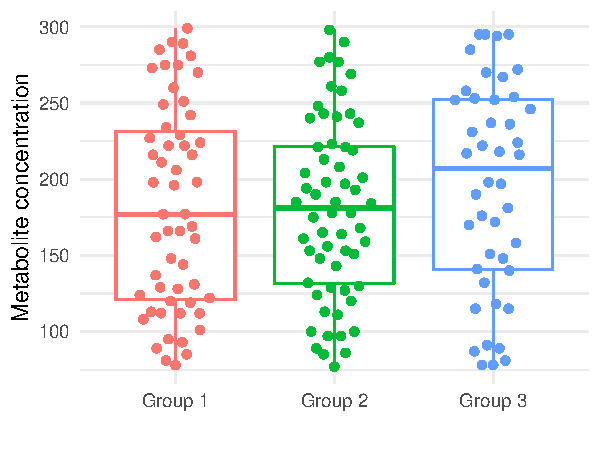
\includegraphics{SN_templates_files/figure-latex/plot-data-1.pdf}
\caption{\label{fig:plot-data}Weight distribution of clinical trial subjects}
\end{figure}

\hypertarget{methods}{%
\section{Methods}\label{methods}}

The following code was used in section \ref{sec:1} to create the original clinical trial data:

\begin{Shaded}
\begin{Highlighting}[]
\CommentTok{\# create a mock dataset}
\NormalTok{n\_subjs }\OtherTok{\textless{}{-}} \DecValTok{99}
\NormalTok{subjID }\OtherTok{\textless{}{-}} \DecValTok{1}\SpecialCharTok{:}\NormalTok{n\_subjs}

\CommentTok{\# generate 99 random \#s between 1 and 10}
\NormalTok{tmp }\OtherTok{\textless{}{-}} \FunctionTok{floor}\NormalTok{(}\FunctionTok{runif}\NormalTok{(n\_subjs, }\AttributeTok{min =} \DecValTok{0}\NormalTok{, }\AttributeTok{max =} \DecValTok{9}\NormalTok{))}
\CommentTok{\# assign those numbers to any of 3 subject groups}
\NormalTok{fn }\OtherTok{\textless{}{-}} \ControlFlowTok{function}\NormalTok{(x) \{ }
  \ControlFlowTok{if}\NormalTok{ (x }\SpecialCharTok{\textgreater{}=} \DecValTok{6}\NormalTok{) }\StringTok{\textquotesingle{}Group 1\textquotesingle{}} 
  \ControlFlowTok{else} \ControlFlowTok{if}\NormalTok{ (x }\SpecialCharTok{\textgreater{}=} \DecValTok{3}\NormalTok{) }\StringTok{\textquotesingle{}Group 2\textquotesingle{}} 
  \ControlFlowTok{else} \StringTok{\textquotesingle{}Group 3\textquotesingle{}} 
\NormalTok{\}}
\NormalTok{subj\_class }\OtherTok{\textless{}{-}} \FunctionTok{sapply}\NormalTok{(tmp, fn)}

\CommentTok{\# pick random weights between 75 and 300}
\NormalTok{wts }\OtherTok{\textless{}{-}} \FunctionTok{floor}\NormalTok{(}\FunctionTok{runif}\NormalTok{(n\_subjs, }\AttributeTok{min =} \DecValTok{75}\NormalTok{, }\AttributeTok{max =} \DecValTok{300}\NormalTok{))}
\CommentTok{\# combine the data into a table}
\NormalTok{df }\OtherTok{\textless{}{-}} \FunctionTok{data.frame}\NormalTok{(}\AttributeTok{ID =}\NormalTok{ subjID, }\AttributeTok{class =}\NormalTok{ subj\_class, }\AttributeTok{wt =}\NormalTok{ wts)}

\CommentTok{\# display the table, splitting the 99 rows into 3 cols wide}
\NormalTok{tmp }\OtherTok{\textless{}{-}} \FunctionTok{cbind}\NormalTok{(df[}\DecValTok{1}\SpecialCharTok{:}\DecValTok{33}\NormalTok{,], }\FunctionTok{rep}\NormalTok{(}\StringTok{\textquotesingle{}|\textquotesingle{}}\NormalTok{, }\DecValTok{33}\NormalTok{), }
\NormalTok{             df[}\DecValTok{34}\SpecialCharTok{:}\DecValTok{66}\NormalTok{,], }\FunctionTok{rep}\NormalTok{(}\StringTok{\textquotesingle{}|\textquotesingle{}}\NormalTok{, }\DecValTok{33}\NormalTok{), }
\NormalTok{             df[}\DecValTok{67}\SpecialCharTok{:}\DecValTok{99}\NormalTok{,])}
\FunctionTok{names}\NormalTok{(tmp) }\OtherTok{\textless{}{-}} \FunctionTok{c}\NormalTok{(}\StringTok{\textquotesingle{}ID\textquotesingle{}}\NormalTok{, }\StringTok{\textquotesingle{}class\textquotesingle{}}\NormalTok{, }\StringTok{\textquotesingle{}wt\textquotesingle{}}\NormalTok{, }\StringTok{\textquotesingle{}|\textquotesingle{}}\NormalTok{, }\StringTok{\textquotesingle{}ID\textquotesingle{}}\NormalTok{, }\StringTok{\textquotesingle{}class\textquotesingle{}}\NormalTok{, }\StringTok{\textquotesingle{}wt\textquotesingle{}}\NormalTok{, }
                \StringTok{\textquotesingle{}|\textquotesingle{}}\NormalTok{, }\StringTok{\textquotesingle{}ID\textquotesingle{}}\NormalTok{, }\StringTok{\textquotesingle{}class\textquotesingle{}}\NormalTok{, }\StringTok{\textquotesingle{}wt\textquotesingle{}}\NormalTok{)}
\NormalTok{knitr}\SpecialCharTok{::}\FunctionTok{kable}\NormalTok{(tmp, }\AttributeTok{format =} \StringTok{\textquotesingle{}latex\textquotesingle{}}\NormalTok{, }\AttributeTok{booktabs =} \ConstantTok{TRUE}\NormalTok{, }
             \AttributeTok{caption =} \StringTok{"Original subject data"}\NormalTok{)}
\end{Highlighting}
\end{Shaded}

The following code was used in section \ref{sec:2} to plot the data:

\begin{Shaded}
\begin{Highlighting}[]
\NormalTok{final\_data }\SpecialCharTok{\%\textgreater{}\%} 
  \FunctionTok{ggplot}\NormalTok{(}\FunctionTok{aes}\NormalTok{(}\AttributeTok{x =}\NormalTok{ class, }\AttributeTok{y =}\NormalTok{ wt, }\AttributeTok{color =}\NormalTok{ class)) }\SpecialCharTok{+}
  \FunctionTok{geom\_boxplot}\NormalTok{() }\SpecialCharTok{+}
  \FunctionTok{geom\_jitter}\NormalTok{(}\AttributeTok{width =} \FloatTok{0.25}\NormalTok{) }\SpecialCharTok{+} 
  \FunctionTok{xlab}\NormalTok{(}\StringTok{""}\NormalTok{) }\SpecialCharTok{+}
  \FunctionTok{ylab}\NormalTok{(}\StringTok{"Weight"}\NormalTok{) }\SpecialCharTok{+} 
  \FunctionTok{theme\_minimal}\NormalTok{() }\SpecialCharTok{+}
  \FunctionTok{theme}\NormalTok{(}\AttributeTok{legend.position =} \StringTok{"none"}\NormalTok{)}
\end{Highlighting}
\end{Shaded}

\hypertarget{references}{%
\section*{References}\label{references}}
\addcontentsline{toc}{section}{References}

\hypertarget{refs}{}
\begin{CSLReferences}{1}{0}
\leavevmode\vadjust pre{\hypertarget{ref-argelaguet_computational_2021}{}}%
Argelaguet, Ricard, Anna S. E. Cuomo, Oliver Stegle, and John C. Marioni. 2021. {``Computational Principles and Challenges in Single-Cell Data Integration.''} \emph{Nature Biotechnology}, May, 1--14. \url{https://doi.org/10.1038/s41587-021-00895-7}.

\leavevmode\vadjust pre{\hypertarget{ref-fisch_omics_2015}{}}%
Fisch, K. M., T. Meissner, L. Gioia, J.-C. Ducom, T. M. Carland, S. Loguercio, and A. I. Su. 2015. {``Omics {Pipe}: A Community-Based Framework for Reproducible Multi-Omics Data Analysis.''} \emph{Bioinformatics} 31 (11): 1724--28. \url{https://doi.org/10.1093/bioinformatics/btv061}.

\leavevmode\vadjust pre{\hypertarget{ref-le_cao_community-wide_2021}{}}%
Lê Cao, Kim-Anh, Al J. Abadi, Emily F. Davis-Marcisak, Lauren Hsu, Arshi Arora, Alexis Coullomb, Atul Deshpande, et al. 2021. {``Community-Wide Hackathons to Identify Central Themes in Single-Cell Multi-Omics.''} \emph{Genome Biology} 22 (1): 220. \url{https://doi.org/10.1186/s13059-021-02433-9}.

\leavevmode\vadjust pre{\hypertarget{ref-perkel2020}{}}%
Perkel, Jeffrey M. 2020. {``Streamline Your Writing {\textemdash} and Collaborations {\textemdash} with These Reference Managers.''} \emph{Nature} 585 (7823): 149--50. \url{https://doi.org/10.1038/d41586-020-02491-2}.

\end{CSLReferences}


\bibliographystyle{spbasic}
\bibliography{bibliography.bib}


\end{document}
